\section{Abbildungen -- Linsen}

\subsection{Konstruktions-Anweisung}

Man benutzt zwei der drei Hauptstrahlen:

\begin{ctabular}{l l >{\textrightarrow}c l}
    1. & Parallel Strahl & & Brennpunkt \\
    2. & Mittelpunkt Strahl & & mit gleichem Winkel zurück \\
    3. & Brennpunkt Strahl & & Paralleler Strahl
\end{ctabular}

\begin{minipage}{0.48\columnwidth}
    \centering
    \textbf{Reelles Bild}

    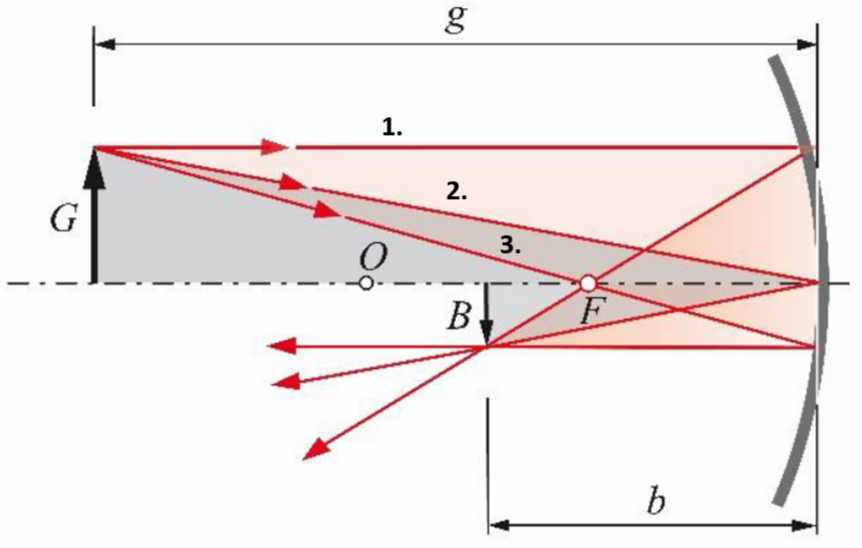
\includegraphics[width= 0.9\columnwidth]{images/reelles_bild.png}
\end{minipage}
\hfill
\begin{minipage}{0.48\columnwidth}
    \centering
    \textbf{Virtuelles Bild}

    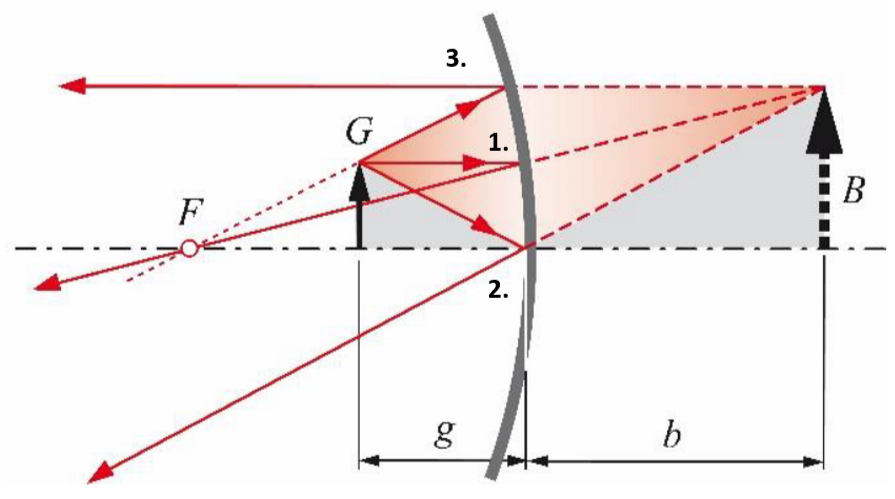
\includegraphics[width= 0.9\columnwidth]{images/virtuelles_bild.png}
\end{minipage}

$B$ wird als \textbf{reeller Bildpunkt} bezeichnet, wenn sich die austretenden Strahlen schneiden.

\smallskip
$B$ wird als \textbf{virtueller Bildpunkt} bezeichnet, wenn sich nur die Verlängerungen der austretenden Strahlen schneiden. 


\subsubsection{Terminologie}

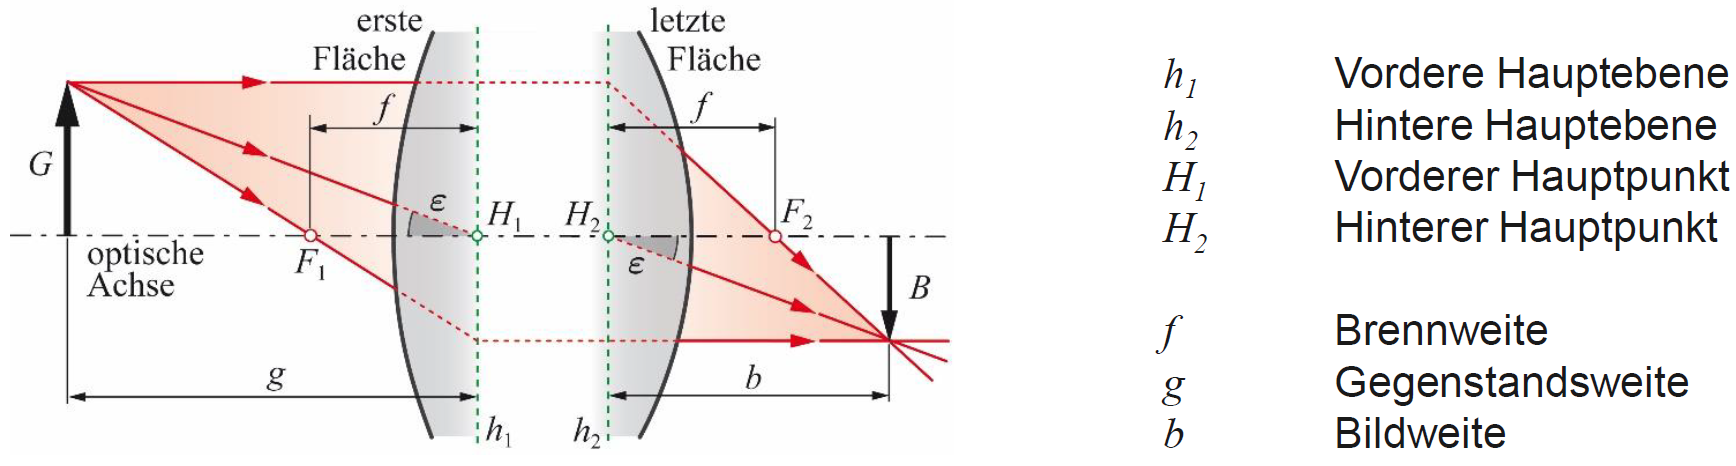
\includegraphics[width=0.9\columnwidth]{images/terminologie.png}

Die \textbf{Öffnungsblende} oder \textbf{Aperturblende} bergrenz das in das System einfallende Lichtbündel

\smallskip
Die \textbf{Feldblende} begrenzt das Bildfeld. Sie legt den Ausschnitt der Objektebene fest, der abgebildet wird.


\example{Abbildungen bei zwei Sammellinsen}

\begin{minipage}{0.48\columnwidth}
    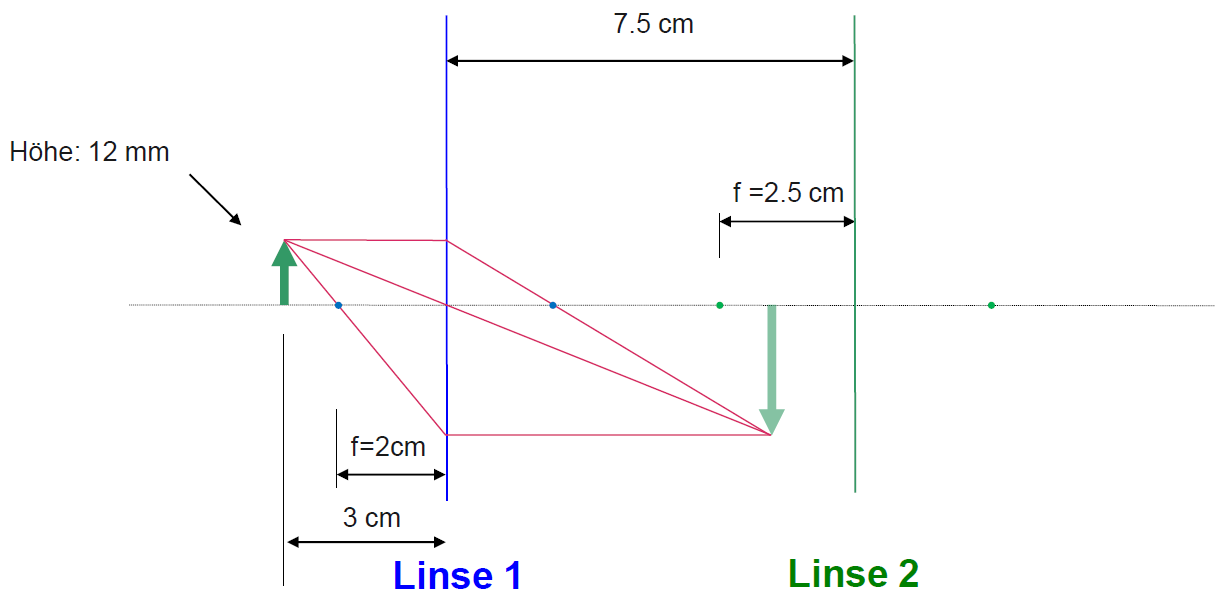
\includegraphics[width=\columnwidth]{images/zwei_sammellinsen_1.png}
\end{minipage}
\hfill
\begin{minipage}{0.48\columnwidth}
    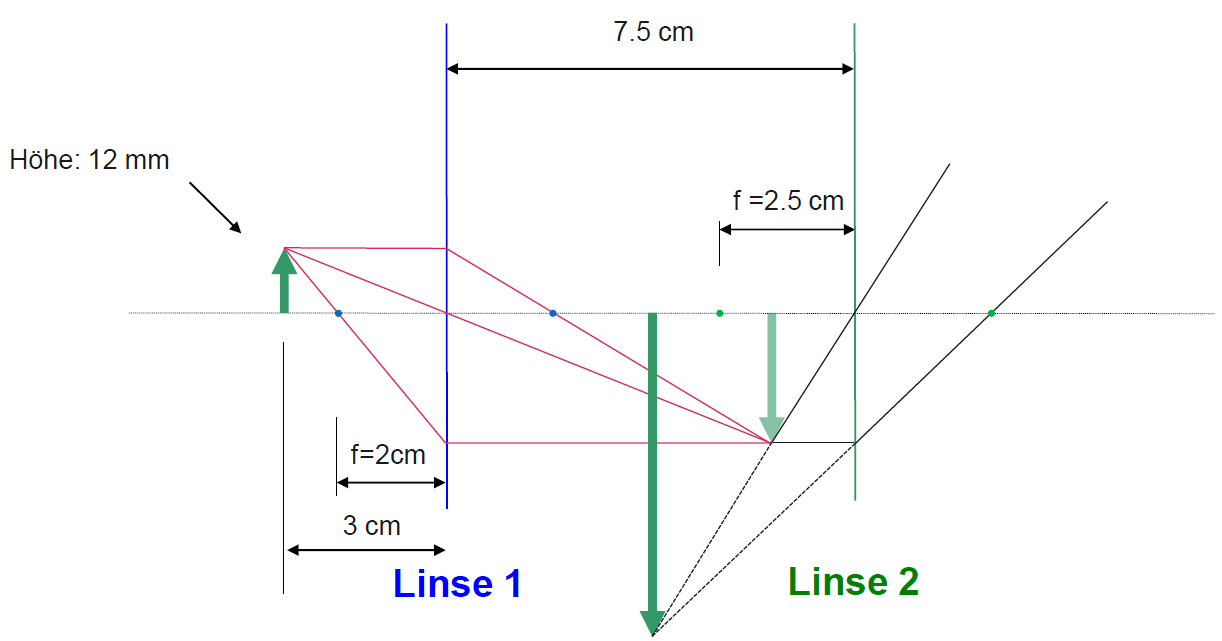
\includegraphics[width=\columnwidth]{images/zwei_sammellinsen_2.png}
\end{minipage}


\subsection{Abbildungsgleichungen}

\textbf{Ein Bild ist scharf dargestellt, wenn die Abbildungsgleichung erfüllt ist!}

\medskip

\begin{minipage}{0.48\columnwidth}
    \paragraph{Abbildungsgleichung}
    $$ \boxed{ \frac{1}{b} + \frac{1}{g} = \frac{1}{f} } $$
\end{minipage}
\hfill
\begin{minipage}{0.48\columnwidth}
    \paragraph{Newtonsche Abb.-Gleichung}
    $$ \boxed{ x_b \cdot x_g = f^2 } $$
\end{minipage}

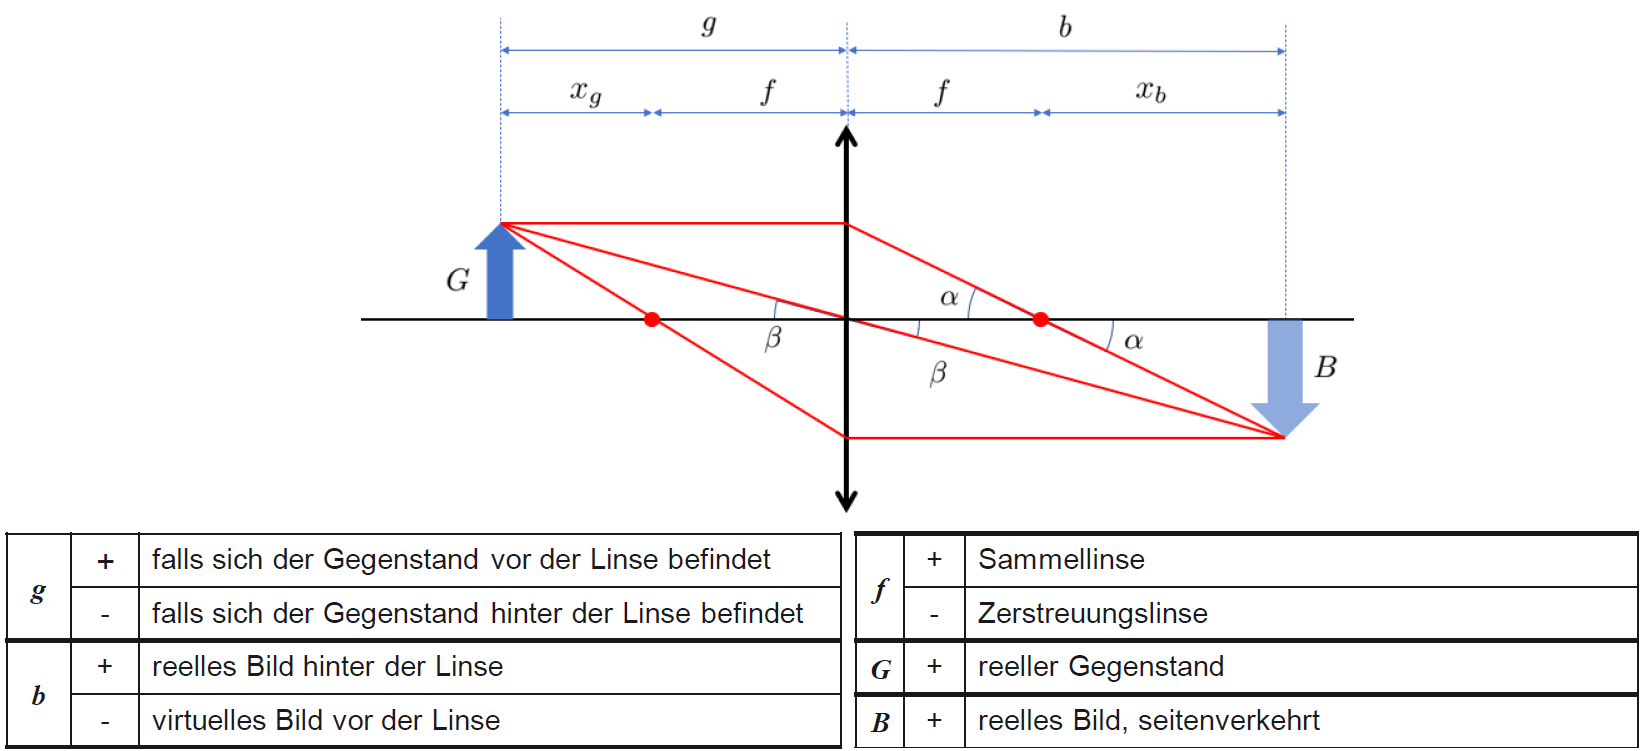
\includegraphics[width=\columnwidth]{images/abbildungsgleichung.png}



\textcolor{blue}{\textbf{Hinweis:} Ein Spiegel hat eine Brennweite von $f = \infty$ \\
\textrightarrow\  Vereinfachung der Abbildungsgleichung!}


\subsubsection{Vergrösserungsverhältnis}

\begin{minipage}{0.35\columnwidth}
    $$ \boxed{ V = \frac{B}{G} = \frac{b}{g} } $$
    $$ \boxed{ V_{\rm tot} = V_1 \cdot V_2 } $$ 
\end{minipage}
\hfill
\begin{minipage}{0.6\columnwidth}
    \begin{tabular}{c l c}
        $V$ & Vergrösserungsverhältnis  & $[V] = 1$         \\
        $b$ & Bildweite                 & $[b] = \meter$    \\
        $g$ & Gegenstandsweite          & $[g] = \meter$    \\
        $B$ & Bildgrösse                & $[B] = \meter$    \\
        $G$ & Gegenstandsgrösse         & $[G] = \meter$    \\
        $f$ & Brennweite                & $[f] = \meter$ 
    \end{tabular}
\end{minipage}



\subsection[Brechkraft]{Brechkraft $\bm{D}$}

\begin{minipage}[t]{0.65\columnwidth}
    Die Optiker benutzen nicht die Brennweite sondern die Brechkraft in \textbf{Dioptrie}  \\
    Es gilt: $1 \, \mathrm{dpt} = 1 \, \reciprocal\meter$
\end{minipage}
\hfill
\begin{minipage}[t]{0.25\columnwidth}
    $$ \boxed{ D = \frac{1}{f} }$$
\end{minipage}






\subsection{Linsenschleifergleichung}

\begin{minipage}[t]{0.52\columnwidth}
    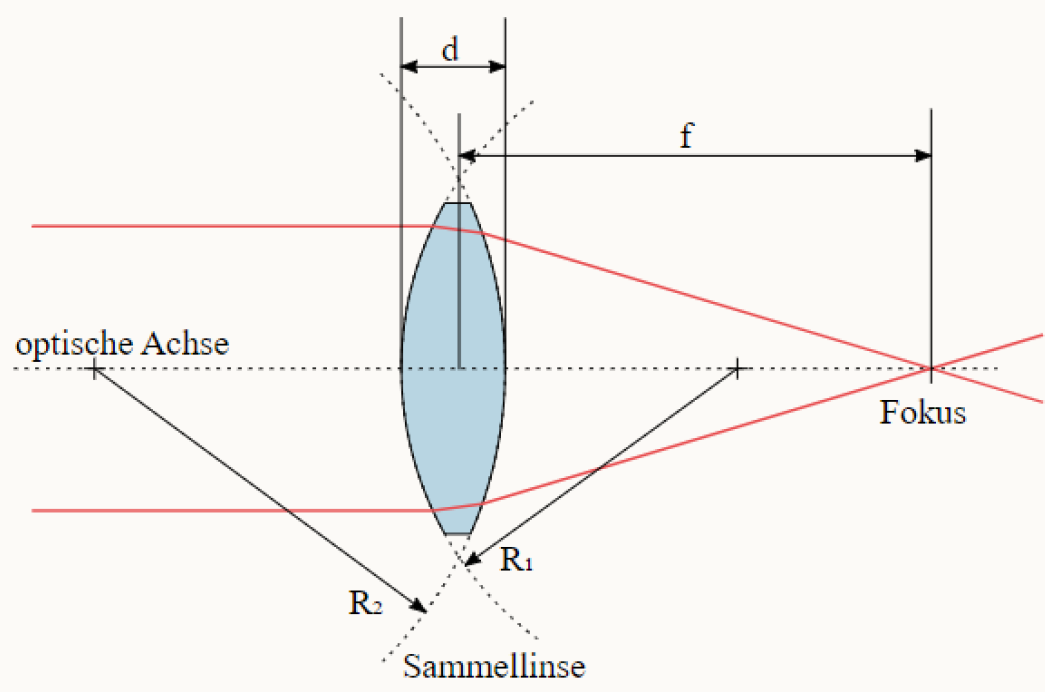
\includegraphics[width=\columnwidth, align=t]{images/Linsenschleifergleichung.png}
\end{minipage}
\hfill
\begin{minipage}[t]{0.46\columnwidth}
    $$\boxed{D = \left( \frac{n_2}{n_1} - 1 \right)  \left(  \frac{1}{R_1} - \frac{1}{R_2} \right) }$$

    \cbl{\textbf{Achtung:} Vorzeichen von $R_i$ beachten!} 

    \raggedright%
    Beide haben gleiches Vorzeichen, wenn Krümmungsmittelpunkte auf gleicher Seite der Linse liegen
\end{minipage}


\subsubsection{Symmetrische Linsen ($\bm{R_1 = R_2}$)}

Für symmetrische Linsen gilt:

\smallskip

\begin{minipage}{0.48\columnwidth}
    $$\boxed{D = (n - 1)\frac{2}{R}}$$
    $$\boxed{f = \frac{1}{D} = \frac{R}{2}\frac{1}{(n - 1)}} $$
\end{minipage}
\hfill
\begin{minipage}{0.48\columnwidth}
    \begin{tabular}{c l c}
        $D$     & Brechkraft        & $[D] = \mathrm{dpt}$                  \\
        $f$     & Brennweite        & $[f] = \frac{1}{\second} = \hertz$    \\
        $R_i$   & Linsenradius      & $[R_i] = \meter$                      \\
        $n$     & Brechungsindex    & $[n] = 1$
    \end{tabular}
\end{minipage}




\subsubsection{Kombination von zwei dünnen Linsen ohne Zwischenraum}

Die Kombination von zwei dünnen Linsen ohne Zwischenraum ist wie folgt definiert:

$$ \boxed{D = D_1 + D_2} $$


\subsection{Konvexe und Konkave Linsen}

\begin{description}
    \item[Konvex:] nach aussen gewölbt \textrightarrow\ Sammellinsen
    \item[Konkav:] nach innen gewölbt \textrightarrow\ Zerstreuungslinsen
\end{description}

\vspace{-0.2cm}

\begin{center}
    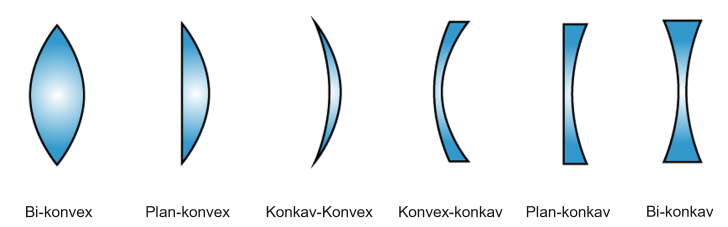
\includegraphics[width=0.9\columnwidth]{images/Konvex.png}
\end{center}

\vspace{-0.2cm}


\subsection{Aberration}

Unter dem Begriff Aberration versteht man die Abweichung vom idealisierten Fall.

\begin{center}
    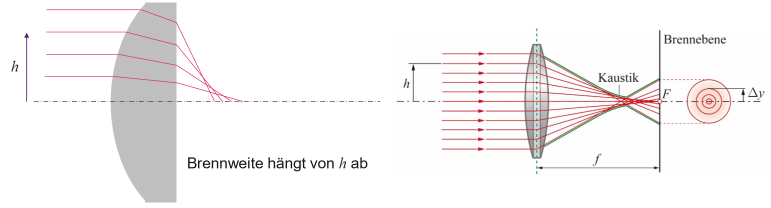
\includegraphics[width=0.9\columnwidth]{images/Aberration.png}
\end{center}



\subsubsection{Astigmatismus}

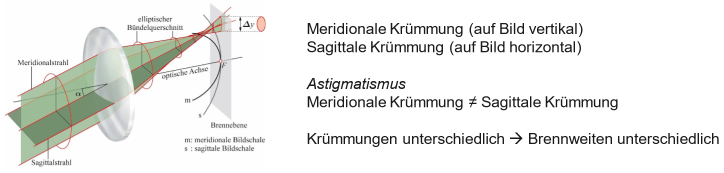
\includegraphics[width=0.9\columnwidth]{images/Astigmatismus.png}


\subsection{Polarisation}

\subsubsection{Lineare Polarisation}

\begin{outline}
    \1 $E_x$ und $E_y$ können \textbf{unterschiedliche Amplituden} haben
    \1 Die \textbf{Phasen müssen gleich} sein.
\end{outline}

\medskip


\begin{minipage}{0.4\columnwidth}
    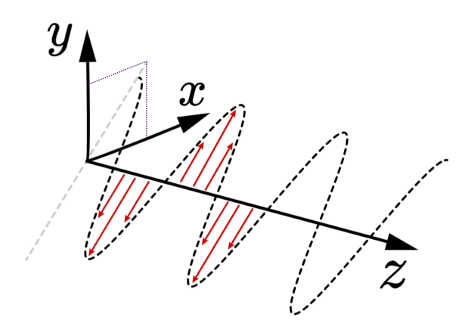
\includegraphics[width=\columnwidth]{images/lineare_Polarisation.png}
\end{minipage}
\hfill
\begin{minipage}{0.58\columnwidth}
    EM-Wellen können mit dem Herzschen Gitter oder mit dem \textbf{Brewster Winkel} linear Polarisiert werden.
    $$ \boxed{  \vec{E} = \begin{pmatrix} E_x \\  E_y \\  0  \end{pmatrix}  } $$
    \begin{center}
        $\vec{E}$ kann zu $\vec{0}$ werden 
    \end{center}
\end{minipage}


\subsubsection{Brewster Winkel}

\begin{minipage}{0.38\columnwidth}
    \textbf{Achtung:} Es gilt $n_1 < n_2$

    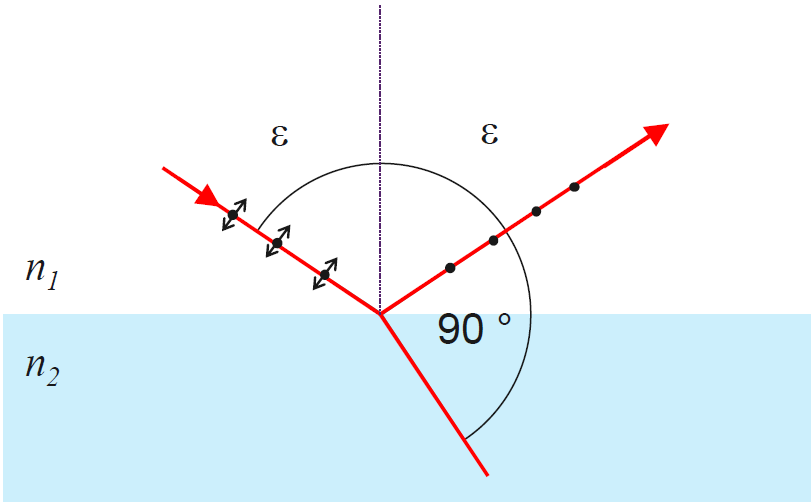
\includegraphics[width=\columnwidth]{images/brewster_winkel.png}
\end{minipage}
\hfill
\begin{minipage}{0.6\columnwidth}
    Unter dem \textbf{Brewster Winkel} wird nur \textbf{linear polarisiertes Licht} zurückgeworfen. 

    Der ins Medium 2 eindringende Strahl steht dabei \textbf{senkrecht} auf dem reflektierten Strahl
    $$ \boxed{  \tan(\varepsilon) = \frac{n_2}{n_1}  }$$
\end{minipage}


\subsubsection{Zirkulare Polarisation}

\begin{outline}
    \1 $x$ und $y$ Komponenten haben die \textbf{gleiche Amplitude}
    \1 \textbf{Phasendifferenz von 90°} 
\end{outline}

\smallskip

\begin{minipage}{0.38\columnwidth}
    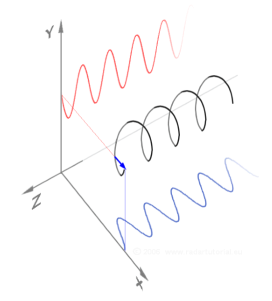
\includegraphics[width=\columnwidth]{images/Zirkulare_Polarisation.png}
\end{minipage}
\hfill
\begin{minipage}{0.58\columnwidth}
    Positive zirkulare Polarisation $\sigma ^+$ \\
    Positive zirkulare Polarisation $\sigma ^-$ 

    $$ \boxed{ \vec{E} = \begin{pmatrix} E_0 \cos(2 \pi ft-kz) \\ E_0 \sin(2 \pi ft -kz) \\ 0 \end{pmatrix}  } $$

    \begin{center}
        $\vec{E}$ kann nicht zu $\vec{0}$ werden 
    \end{center}  
\end{minipage}


\subsubsection{Elliptische Polarisation}

\vspace{-0.2cm}

\begin{minipage}[c]{0.58\columnwidth}
    \begin{outline}
        \1 $x$ und $y$ Komponenten haben \textbf{unterschiedliche Amplituden}
        \1 \textbf{beliebige Phasendifferenz}
    \end{outline}
\end{minipage}
\hfill
\begin{minipage}[c]{0.4\columnwidth}
    $$ \boxed{  \vec{E} = 
    \begin{pmatrix} 
        E_0 \cos(2 \pi ft-kz) \\ 
        E_0 \cos(2 \pi ft -kz + \varphi) \\ 
        0 
    \end{pmatrix}  } $$
\end{minipage}


\subsubsection{Doppelbrechung}

Doppelbrechung ist eine anisotropische Eigenschaft von Kristrallen \\
Diese Kristalle haben unterschiedliche Brechungsindizes in unterschiedliche Richtungen 

\smallskip

Nach einer gewissen Zeit $t$ haben die $x$- und $y$-Komponente einen Phasenunterschied. \\
\textrightarrow\  $x$ und $y$ bewegen sich unterschiedlich schnell fort 

\begin{center}
    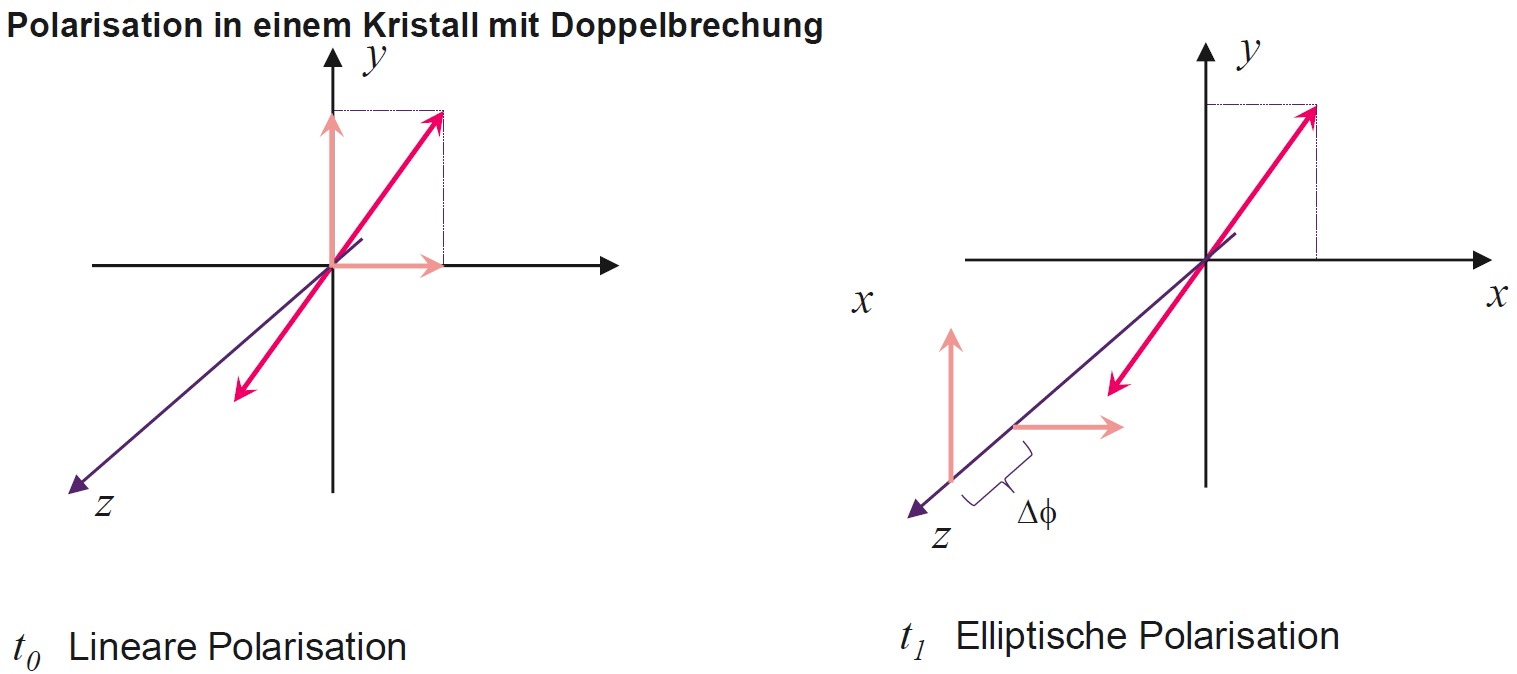
\includegraphics[width=0.8\columnwidth]{images/kristall_mit_doppelbrechung.png}
\end{center}

\vspace{-0.2cm}


\subsection{Streuung}

\subsubsection{Diffuse Streuung}

Streuung des Lichts an Teilchen von Dimensionen $d \gg \lambda$ 

\begin{minipage}{0.45\columnwidth}
    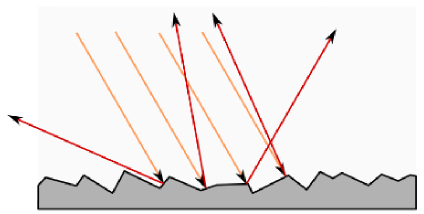
\includegraphics[width=\columnwidth]{images/diffuse_streuung.jpg}
\end{minipage}
\hfill
\begin{minipage}{0.53\columnwidth}
    \begin{itemize}
        \item Licht als \textbf{Strahlen}
        \item Reflexion in alle Richtungen
        \item Keine bevorzugte Richtung \\
            unabhängig von $\lambda$ 
        \item Wolken, Nebel 
        \item milchiche Lösungen 	  
    \end{itemize}
\end{minipage}


\subsubsection{Rayleigh-Streuung}

Streuung des Lichts an Teilchen von Dimensionen $d < \lambda$ (atomare Grösse)

\smallskip

\begin{minipage}{0.34\columnwidth}
    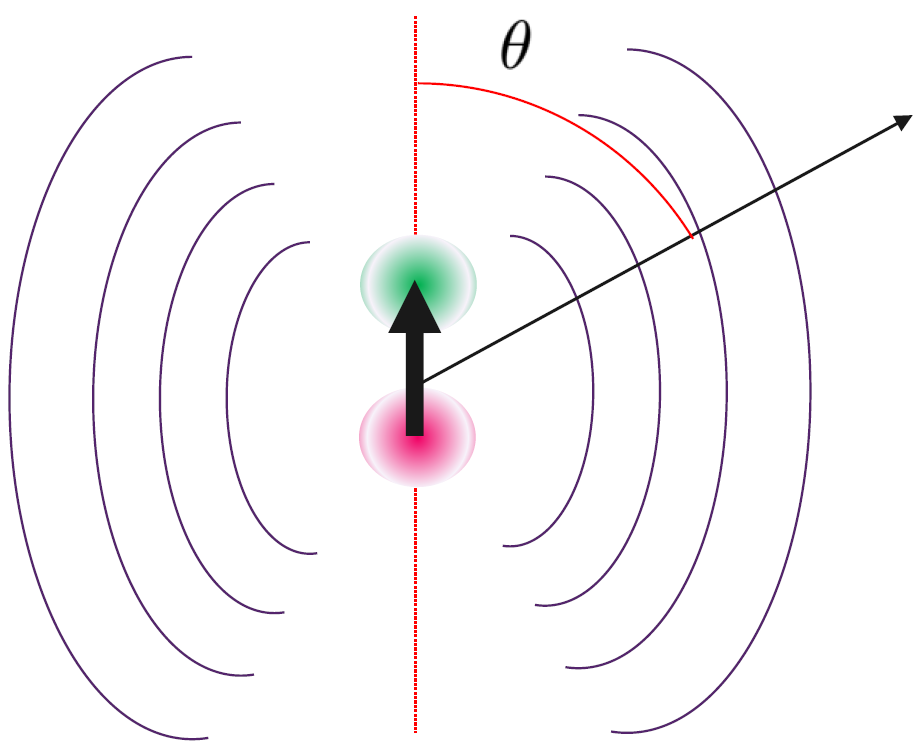
\includegraphics[width=\columnwidth]{images/rayleigh_streuung.png}
\end{minipage}
\hfill
\begin{minipage}{0.64\columnwidth}
    $$ \boxed{ I(\theta) = A \, f^4 \, \frac{\sin^2 (\theta)}{r^2} } $$

    \textrightarrow\  hochfrequentes Licht wird viel stärker abgestrahlt!

    \begin{itemize}
        \item Licht als \textbf{Wellen} senkrecht zur Ausbreitungsrichtung 
        \item Abstrahlmuster eines Dipols
        \item Himmel tagsüber blau 
        \item Himmel abends rötlich	  
    \end{itemize}
\end{minipage}

